\documentclass[12pt]{article}
\usepackage{graphicx}
\usepackage{caption}

\title{High Resolution Time of Flight Mass Spectrometer for Measuring Products in Heterogeneous Catalysis in Highly Sensitive Microreactors}
\author{Thomas, Robert, etc.}
\date{\today}

\begin{document}
\maketitle

\begin{abstract}
We demonstrate that high resolution time of flight mass spectrometry can be successfully applied to detect gas-phase product in heterogeneous catalysis. Combining the instrument with the highly sensitive microreactors opens the possibility to measure on system that are otherwise difficult due to ....
\end{abstract}

\section{Introduction}
Something about the relevance of this system. Catalysis is interesting because... Typical problems with QMS approach. 

\section{System design}
The complete system enables high sensitivity reactivity measurements of the catalyst under investigation combined with high resolution mass spectrometry. The catalyst under investigation is deposited in a microcreactor from where the products are detected with time of flight mass spectrometry. A schematic of the entire setup is shown in Figure \ref{fig:TOF_microreactor}
\begin{center}
	\includegraphics[scale=0.60]{TOF_microreactor.png}
	\captionof{figure}{Schematic of the total system (not to scale)}
	\label{fig:TOF_microreactor}
\end{center}

\subsection{Microreactor and gas handling}

\subsubsection{The microreactor platform}
Catalysts testing were performed in a microreactor platform \cite{Henriksen2009}. The microreactors are fabricated in silicon and measures 20x15\,mm. The reactor consists of two gas inlets, a gas outlet, a reactor volume and a capillary used for probing the gas from the reactor volume. The reactor volume is 3\,$\mu$m deep and 1 cm in diameter resulting in a 240\,nL volume. The two gas inlets are combined on the chip where the inlet gases mix by diffusion. The capillary is designed such that approximately $3\cdot10^{14}$\,molecules$\cdot$s$^{-1}$ is probed from the reactor volume. Any surplus of gas from the two inlets that does not enter the reactor volume is directed through the outlet into a turbo pump. The design ensures that all molecules entering the reactor volume hence exposed to the catalyst under investigation is detected giving the system high sensitivity.

The microreactor is heated by joule heating of a 50 nm platinum strip evaporated through a shadow mask on the backside of the chip. The heating element is contacted by two pogo pins which is connected to a power supply. Additionally, two extra contacts are placed on the chip which facilitates 4 wire measurement of the resistance of the heating element. The heating strip is hence used as a resistance temperature detector (RTD) to monitor the temperature of the chip. At the current configuration temperatures from room temperature to approximately 450\,$^{\circ}$C can be reached.


\subsubsection{Gas handling}
The two gas inlets on the microreactor chip is connected to a gas handling system. A total of 6 gases with accompanying flow controllers are used to control the inlet gas. Currently, the system is configured in a 4+2 setup where 4 gases are connected to the one inlet and to gases on the other inlet. All valves and flow controllers are interfaced to computer enabling remote control of the system and the possibility to run experiments over several days without human intervention.

\subsection{Time of flight}
The time of flight equipment used for detection of gas molecules flowed through the capillary of the microreactor is designed as an orthogonal mass spectrometer. Ionized ions enter the source through a series of Einzel lenses used for focusing the beam minimizing divergence. In the source they are pushed into the flight tube by an the initial push voltage, V$_p$. The ions are further accelerated from ground potential to the liner potential, V$_L$, which is the drift voltage of the flight tube. At the end of the flight tube a reflectron is installed which have two primary purposes. The effective drift length is increased hence increasing resolution of the equipment. The reflectron also works as a focusing lens compensating for any initial velocity dispersion of the ions, i.e. ions with an initial higher velocity will have an increased flight length compared to slower ions. The microchannel plate (MCP) used for detection is placed in the focal point of the reflectron giving maximum compensation for initial velocity dispersion. The theoretical resolution of the equipment is $\Delta$m/m$\sim$4000.

\subsubsection{Ionization of gas}
As ionization source of the gas flow from the microreactor capillary an modified Bayard-Alpert ion gauge is used. 

\section{Test system}
Ammonia oxidation

\section{Summary}

\section{Acknowledgements}

\bibliographystyle{unsrt}
\bibliography{literature}

\end{document}
